\chapter{Calcul des coefficients pour un cylindre infini}
\label{sec:cylindre}
\minitoc
\newpage
\sectionstar{Introduction}
L'introduction de courbure dans les CIOE est d'un atout majeur, car les objets réels sont rarement localement plat, mais plutôt de type sphère-cone. Nous allons présentons dans cette partie l'introduction d'une courbure dans une seule direction.

\section{Cas d'un objet cylindrique}

  % On rappelle les formules des opérateurs \(\vdiv, \vrot\) en coordonnée cylindrique \((r,\theta,z)\).
  % \begin{align}
  %   \vrot \vect{V} &= \left(\frac{1}{r}\ddr{\theta}{V_z} - \ddr{z}{V_\theta}\right)\vect{e_r} +
  %   \left(\ddr{z}{V_r} - \ddr{r}{V_z}\right)\vect{e_\theta} +
  %   \frac{1}{r}\left(\ddr{r}{(rV_\theta)}-\ddr{\theta}{V_r}\right)\vect{e_z}
  %   \\
  %   \vdiv \vect{V} &= \frac{1}{r}\ddr{r}{(rV_r)}+\frac{1}{r}\ddr{\theta}{V_\theta}+\ddr{z}{V_z}
  %   \\
  %   \vgrad f &= \ddr{r}{f}\vect{e_r}
  %   +\frac{1}{r}\ddr{\theta}{f}\vect{e_\theta} + \ddr{z}{f}\vect{e_z}
  % \end{align}

  \begin{figure}[!hbt]
    \centering
    \tikzsetnextfilename{cylindre_1_couche}
    \begin{tikzpicture}
      \coordinate (mat) at (0,-1.5);
\coordinate (vide) at (0,-2);
\coordinate (c) at (0,0);

\fill [lightgray] (c) circle (2);
\fill [white] (c) circle (1.5);
\fill [pattern=north east lines] (c) circle (1.5);

\draw (c) circle (2);
\draw (c) circle (1.5);


\coordinate (n) at (0,2);

%\draw (vide) node [below] {$\eps_0,\mu_0$};
\draw (mat) node [below] {$\peps,\pmu$};

% Axess
\draw [->] (n) -- ++(0,1) node [at end, right] {$\v{\mr}$};
\draw [->] (n) -- ++(1,0) node [at end, right] {$\v{\mt}$};

\draw (n) ++(0.2,0.2) circle(0.1cm) node [above=0.1cm] {$\v{\mz}$};
\draw (n) ++(0.2,0.2) +(135:0.1cm) -- +(315:0.1cm);
\draw (n) ++(0.2,0.2) +(45:0.1cm) -- +(225:0.1cm);

%\draw [->>,thick] (lt) ++ (1,1) -- (mt) ;


    \end{tikzpicture}
  \end{figure}

  On exprime les équations de Maxwell dans le matériau dans la base cylindrique et sans pertes de généralité, on peut réaliser une transformée de Fourier en \(z\) par invariance en translation et en \(\theta\) par invariance en rotation.
  Cependant, le multiplicateur de Fourier associé à la coordonnée \(\theta\) doit être un entier pour assurer la périodicité. On le note \(n\).

  \begin{equation}
    \vE(r,\theta,z) = \frac{1}{2\pi}\sum_{n=-\infty}^{\infty}\int_{\RR} e^{i(n \theta + k_z z )}\hat{\vE} (r,n,k_z) \dd{k_z}
  \end{equation}

  \begin{prop}
    Soit
    \begin{equation}
      k_3 = \sqrt{\w^2\eps\mu - k_z^2}
    \end{equation}
    et \(J_n(z)\) et \(H_n^{(2)}(z)\) des solutions de l'équation de Bessel d'ordre \(n\).

    Alors \(\exists (c_i(n,k_z))_{1<=i<=4} \in \CC(\NN\times\RR)^4\) tels que
    \begin{subequations}
      \begin{align}
        \hat{E_z}(r,n,k_z) &= c_1(n,k_z) J_n\left(k_3r\right) + c_2(n,k_z) H_n^{(2)}\left(k_3r\right)
        \\
        \hat{H_z}(r,n,k_z) &= c_3(n,k_z) J_n\left(k_3r\right) + c_4(n,k_z) H_n^{(2)}\left(k_3r\right)
      \end{align}
    \end{subequations}
  \end{prop}

  \begin{proof}

    On peut simplifier les opérateurs différentiels:

    \begin{align}
      \vrot \hat \vE(r,n,k_z) &= i\left(\frac{n}{r}\hat{E_z} - k_z\hat{E_\theta}\right)\vect{e_r} +
      \left(ik_z\hat{E_r} - \ddr{r}{\hat{E_z}}\right)\vect{e_\theta} +
      \frac{1}{r}\left(\ddr{r}{(r\hat{E_\theta})}-in\hat{E_r}\right)\vect{e_z}
      \\
      &=-i\w\mu \hat \vH(r,n,k_z)
    \end{align}

    On remarque que la méthode utilisée pour le plan aboutie à une équation différentielle à coefficients non constants de type \(r\ddr{r}{\vect{X}}(r,n,k_z) = \mat{M}(r,n,k_z)\vect{X}(r,n,k_z)\).
    On ne peut pas exprimer la solution avec les valeurs et vecteurs propres de la matrice.
    %Nous allons donc trouver une équation de Bessel en développant le système de Maxwell.

    Comme l'on cherche \(\hat \vE_t, \hat \vH_t\), on remarque que les 2\ieme composantes des équations de Maxwell permettent de déduire \(\hat\vE_t, \hat\vH_t\) de \( \hat E_z, \hat H_z\).

    On couple les 2 équations du système de Maxwell pour aboutir à une équation sur \(\hat \vE\) seul:

    % \begin{align}
    %   \vrot \vrot \hat \vE &= \w^2\eps\mu \hat \vE
    %   \\
    %   \vdiv \hat \vE &= 0
    % \end{align}

    % \begin{multline}
    %   \vrot \vrot \hat \vE = \dots\\
    %   i\left(\frac{n}{r^2}\left(\ddr{r}{(r\hat{E_\theta})} - in\hat{E_r}\right) - k_z\left(ik_z\hat{E_r} - \ddr{r}{\hat{E_z}}\right)\right)  \vect{e_r} \dots\\
    %   + \left(-k_z\left(\frac{n}{r}\hat{E_z} - k_z\hat{E_\theta}\right) -\ddr{r}{}\left(\frac{1}{r}\left(\ddr{r}{(r\hat{E_\theta})}-in\hat{E_r}\right)\right)\right)  \vect{e_\theta} \dots\\
    %   + \frac{1}{r}\left(\ddr{r}{} \left(r\left(ik_z\hat{E_r} - \ddr{r}{\hat{E_z}}\right)\right) + n \left(\frac{n}{r}\hat{E_z} - k_z\hat{E_\theta}\right)\right) \vect{e_z}
    % \end{multline}

    % On aboutit au système suivant
    \begin{equation}
      \left\lbrace
      \begin{array}{ccc}
        -\left(\w^2\eps\mu -\frac{n^2}{r^2}  - k_z^2\right)\hat{E_r}  +i\frac{n}{r^2}\ddr{r}{(r\hat{E_\theta})}  +k_z\ddr{r}{\hat{E_z}} & = & 0\\
        in\ddr{r}{}\left(\frac{\hat{E_r}}{r}\right) -\left(\w^2\eps\mu - k_z^2\right)\hat{E_\theta} + \ddr{r}{}\left(\frac{1}{r}\ddr{r}{(r\hat{E_\theta})}\right)  - n\frac{k_z}{r}\hat{E_z} & = & 0\\
        i\frac{k_z}{r}\ddr{r}{(r\hat{E_r})}  - n\frac{k_z}{r}\hat{E_\theta}  -\left(\w^2\eps\mu - \frac{n^2}{r^2} \right)\hat{E_z} - \frac{1}{r}\ddr{r}{}\left(r\ddr{r}{\hat{E_z}}\right) & = & 0
      \end{array}
      \right.
    \end{equation}

    De la troisième  équation, on trouve pour \(r\not=0\)
    \begin{equation}
    r^2 \ddr[2]{r}{\hat{E_z}} + r\ddr{r}{\hat{E_z}} + \left(r^2\w^2\eps\mu - n^2\right)\hat{E_z} =ik_zr\ddr{r}{(r\hat{E_r})} -  nk_zr\hat{E_\theta}
    \end{equation}

    Or comme \(\vdiv \hat \vE = 0\), on a
    \begin{align}
      \vdiv\hat \vE &= \frac{1}{r}\ddr{r}{(r\hat{E_r})} + \frac{in}{r}\hat{E_\theta} + ik_z\hat{E_z}
      \\
      k_z^2r^2 \hat{E_z} &= ik_zr\ddr{r}{(r\hat{E_r})} - nk_zr\hat{E_\theta}
    \end{align}

    On obtient donc sur la composante \(\hat{E_z}\):
    \begin{equation}
      r^2 \ddr[2]{r}{\hat{E_z}} + r\ddr{r}{\hat{E_z}} + \left(r^2\left(\w^2\eps\mu - k_z^2\right) - n^2\right)\hat{E_z} = 0
    \end{equation}

    C'est une équation de Bessel (cf \cite[eq (6.80)]{bowman_introduction_1958}), dont des solutions générales sont: soient \((c_1,c_2) \in \CC^2\):
     \begin{equation}
      \hat{E_z}(r,n,k_z) = c_1 J_n\left(k_3r\right) + c_2 H_n^{(2)}\left(k_3r\right)
    \end{equation}
    où \(J_n\) est la fonction de Bessel du premier type, \(H_n^{(2)}\) la fonction de Hankel de deuxième type.
    On sait que l'on peut prendre n'importe quel couple de fonctions de Bessel (cf \eqref{eq:annex:bessel:equiv_bessel}), on choisit ce dernier car les \(J_n\) sont régulières et les \(H_n\) évoluent en \(\frac{1}{\sqrt{r}}\) à l'infini, donc ce choix est adapté à une décomposition en une onde incidente partout définie et une onde réfléchie décroissante à l'infini.

    De plus, d'après \cite[p.~358]{abramowitz_handbook_1964}, on sait qu'une fonction de Bessel d'ordre \(n\) est linéairement dépendante de celle d'ordre \(-n\).
    On peut donc se restreindre à \(n\) entier naturel

    On trouve exactement le même résultat pour \(\hat{H_z}\): soient \((c_3,c_4) \in \CC^2\)
    \begin{equation}
      \hat{H_z}(r,n,k_z) = c_3 J_n\left(k_3r\right) + c_4 H_n^{(2)}\left(k_3r\right)
    \end{equation}
  \end{proof}


  \begin{defn}
    On définit les matrices \(\mJ_{E}(r,n,k_z),\mH_{E}(r,n,k_z),\mJ_{H}(r,n,k_z),\mH_{H}(r,n,k_z)\)
    \begin{align}
      \mJ_{E}(r,n,k_z) &=
      \begin{bmatrix}
        -\frac{nk_z}{rk_3^2}J_n(k_3r) & \frac{ik\eta}{k_3}J_n'(k_3r)
        \\
        J_n(k_3r) & 0
      \end{bmatrix}
      \\
      \mH_{E}(r,n,k_z) &=
      \begin{bmatrix}
        -\frac{nk_z}{rk_3^2}H_n^{(2)}(k_3r) & \frac{ik\eta}{k_3}H_n^{(2)}{}'(k_3r)
        \\
        H_n^{(2)}(k_3r) & 0
      \end{bmatrix}
      \\
      \mJ_{H}(r,n,k_z) &=
      \begin{bmatrix}
        0 & -J_n(k_3r)
        \\
        -\frac{ik}{\eta k_3}J_n'(k_3r) & -\frac{nk_z}{rk_3^2}J_n(k_3r)
      \end{bmatrix}
      \\
      \mH_{H}(r,n,k_z) &=
      \begin{bmatrix}
        0 & -H_n^{(2)}(k_3r)
        \\
        -\frac{ik}{\eta k_3}H_n^{(2)}{}'(k_3r) & -\frac{nk_z}{rk_3^2}H_n^{(2)}(k_3r)
      \end{bmatrix}
    \end{align}
  \end{defn}

  \begin{prop}
    Alors les champs tangentiels s'écrivent
    \begin{subequations}
      \begin{align}
        \hat \vE_t(r,n,k_z) &= \mJ_{E}(r,n,k_z)
        \begin{bmatrix}
          c_1 \\
          c_3
        \end{bmatrix}
        +
        \mH_{E}(r,n,k_z)
        \begin{bmatrix}
          c_2 \\
          c_4
        \end{bmatrix}
        \label{eq:imp_fourier:cylindre:Et}\\
        \vect{e_r}\times\hat \vH_t(r,n,k_z) &=
        \mJ_{H}(r,n,k_z)
        \begin{bmatrix}
          c_1 \\
          c_3
        \end{bmatrix}
        +
        \mH_{H}(r,n,k_z)
        \begin{bmatrix}
          c_2 \\
          c_4
        \end{bmatrix}
        \label{eq:imp_fourier:cylindre:Ht}
      \end{align}
    \end{subequations}
  \end{prop}


  \begin{proof}
    À partir des équations de Maxwell restantes, on peut déterminer \(\hat{E_r},\hat{E_\theta},\hat{H_r},\hat{H_\theta}\).
    \begin{equation}
      \left\lbrace
      \begin{matrix}
        -ik_z\hat{E_\theta} + i\w\mu \hat{H_r} = -\frac{in}{r}\hat{E_z}
        \\
        ik_z\hat{E_r} + i\w\mu \hat{H_\theta} = \ddr{r}{\hat{E_z}}
        \\
        i\w\eps \hat{E_r} + ik_z \hat{H_\theta} = \frac{in}{r}\hat{H_z}
        \\
        i\w\eps \hat{E_\theta} - ik_z \hat{H_r} = -\ddr{r}{\hat{H_z}}
      \end{matrix}
      \right.
    \end{equation}

    Cela revient à résoudre \(\vect{Y} = \mat{M}\vect{X}\) où la matrice \(\mat{M}\) et les vecteurs \(\vect{X}, \vect{Y}\) sont définis tels que
    \begin{equation}
      \mat{M} =
      \begin{bmatrix}
      0 & -ik_z & i\w\mu & 0
      \\
      ik_z & 0 & 0 & i\w\mu
      \\
      i\w\eps & 0 & 0 & ik_z
      \\
      0 & i\w\eps & -ik_z & 0
      \end{bmatrix}
      \,
      \vect{X} =
      \begin{bmatrix}
        \hat{E_r}\\
        \hat{E_\theta}\\
        \hat{H_r}\\
        \hat{H_\theta}
      \end{bmatrix}
      \,
      \vect{Y} =
      \begin{bmatrix}
        -\frac{in}{r}\hat{E_z}\\
        \ddr{r}{\hat{E_z}}\\
        \frac{in}{r}\hat{H_z}\\
        -\ddr{r}{\hat{H_z}}
      \end{bmatrix}
    \end{equation}

    On remarque que \(\mM\mM = \left(k_z^2 - \omega^2\eps\mu\right)\mI\) et donc que \(\det(\mat{M}) = \left(ik_3\right)^2\).

    On suppose ce dernier non nul, on peut déduire \(\vect{X}\):

    \begin{equation}
      \begin{bmatrix}
        \hat{E_r}\\
        \hat{E_\theta}\\
        \hat{H_r}\\
        \hat{H_\theta}
      \end{bmatrix} =
      \frac{1}{-k_3^2}
      \begin{bmatrix}
      0 & -ik_z & i\w\mu & 0
      \\
      ik_z & 0 & 0 & i\w\mu
      \\
      i\w\eps & 0 & 0 & ik_z
      \\
      0 & i\w\eps & -ik_z & 0
      \end{bmatrix}
      \begin{bmatrix}
        -\frac{in}{r}\hat{E_z}\\
        \ddr{r}{\hat{E_z}}\\
        \frac{in}{r}\hat{H_z}\\
        -\ddr{r}{\hat{H_z}}
      \end{bmatrix}
    \end{equation}

    On extrait alors \(\hat{E_\theta}, \hat{H_\theta}\) pour obtenir les champs tangentielles à \(\vect{e_r}\) en tout point, sachant déjà \(\hat{E_z}, \hat{H_z}\).

    \begin{align}
      \hat{E_r} & = \frac{1}{k_3^2}\left(ik_z\ddr{r}{\hat{E_z}}+\frac{k\eta n}{r}\hat{H_z}\right)
      \\
      \hat{E_\theta} &= -\frac{1}{k_3^2}\left(\frac{nk_z}{r}\hat{E_z} - i\w\mu\ddr{r}{\hat{H_z}}\right)
      \\
      \hat{E_z} &= c_1 J_n(k_3 r) + c_2 H_n^{(2)}(k_3 r)
      \\
      -\hat{H_z} &= -c_3 J_n(k_3 r) - c_4 H_n^{(2)}(k_3 r)
      \\
      \hat{H_\theta} &= -\frac{1}{k_3^2}\left(i\w\eps\ddr{r}{\hat{E_z}} + \frac{nk_z}{r}\hat{H_z}\right)
    \end{align}

    On dérive les fonctions de Bessel:

     \begin{align}
      \hat{E_\theta} &= -\frac{nk_z}{rk_3^2}\left(c_1J_n(k_3r) + c_2 H_n^{(2)}(k_3r)\right) + \frac{ik\eta}{k_3}\left(c_3J_n'(k_3r) + c_4 H_n^{(2)}{}'(k_3r)\right)
      \\
      \hat{E_z} &= c_1 J_n(k_3 r) + c_2 H_n^{(2)}(k_3 r)
      \\
      -\hat{H_z} &= -c_3 J_n(k_3 r) - c_4 H_n^{(2)}(k_3 r)
      \\
      \hat{H_\theta} &= -\frac{ik}{\eta k_3}\left(c_1J_n'(k_3r) + c_2 H_n^{(2)}{}'(k_3r)\right) - \frac{nk_z}{rk_3^2}\left(c_3J_n(k_3r) + c_4 H_n^{(2)}(k_3r)\right)
    \end{align}

    Et on obtient


    \begin{subequations}
      \label{eq:imp_fourier:cylindre:champs}
      \begin{align}
        \label{eq:imp_fourier:cylindre:champs:E}
        \hat \vE_t(r,n,k_z) &= \mJ_{E}(r)
        \begin{bmatrix}
          c_1 \\
          c_3
        \end{bmatrix}
        +
        \mH_{E}(r)
        \begin{bmatrix}
          c_2 \\
          c_4
        \end{bmatrix}
        \\
        \label{eq:imp_fourier:cylindre:champs:H}
        \vect{e_r}\times\hat \vH_t(r,n,k_z) &=
        \mJ_{H}(r)
        \begin{bmatrix}
          c_1 \\
          c_3
        \end{bmatrix}
        +
        \mH_{H}(r)
        \begin{bmatrix}
          c_2 \\
          c_4
        \end{bmatrix}
      \end{align}
    \end{subequations}

  \end{proof}

  %%%%%%%%%%%%%%%%%%%%%%%%%%%%%%%%%%%%%%%%%%%%%%%%%%%%%%%%%%%%%%%%%%%%%%%%%%%%%%%%%%%%%%%%%%%%%%%%%%%%%%%%
  %%%%%%%%%%%%%%%%%%%%%%%%%%%%%%%%%%%%%%%%%%%%%%%%%%%%%%%%%%%%%%%%%%%%%%%%%%%%%%%%%%%%%%%%%%%%%%%%%%%%%%%%
  %%%%%%%%%%%%%%%%%%%%%%%%%%%%%%%%%%%%%%%%%%%%%%%%%%%%%%%%%%%%%%%%%%%%%%%%%%%%%%%%%%%%%%%%%%%%%%%%%%%%%%%%


  \subsection{Opérateur d'impédance pour une couche}

    Soit \(r_1 = r_0 + d\)
    \begin{defn}
      On définit le symbole \(\hat \mZ(n,k_z)\) de l'opérateur d'impédance la matrice telle que
      \begin{equation}
        \hat \vE_t(r_1,n,k_z) = \hat \mZ(n,k_z) \left(\vect{e_r}\pvect \hat \vH_t(r_1,n,k_z)\right)
      \end{equation}
    \end{defn}

    \begin{thm}
      Si on suppose que les fonctions de Bessel et leurs dérivées ne s’annulent pas en \(k_3r_0\) et que
      la matrice \(\mH_{H}(r_1) - \mJ_{H}(r_1)\mJ_{E}(r_0)^{-1}\mH_{E}(r_0)\) est inversible

      Alors le symbole \(\hat \mZ(n,k_z)\) de l'opérateur d'impédance est
      \begin{multline}
        \hat \mZ(n,k_z) =
        \left(\mH_{E}(r_1)\mH_{E}(r_0)^{-1} - \mJ_{E}(r_1)\mJ_{E}(r_0)^{-1}\right)\\
        \left(\mH_{H}(r_1)\mH_{E}(r_0)^{-1} - \mJ_{H}(r_1)\mJ_{E}(r_0)^{-1}\right)^{-1}
      \end{multline}
    \end{thm}

    \begin{proof}

      On injecte la relation \(\vE_t(r_0,\theta,z) = 0\) équivalente à \(\hat \vE(r_0,n,k_z) = 0\) dans \eqref{eq:imp_fourier:cylindre:Et}.
      \begin{equation}
        \mJ_{E}(r_0)
        \begin{bmatrix}
          c_1 \\
          c_3
        \end{bmatrix}
        =-\mH_{E}(r_0)
        \begin{bmatrix}
          c_2 \\
          c_4
        \end{bmatrix}
      \end{equation}

      Or par définition des matrices,
      \begin{align}
        \det(\mJ_E(r_0)) &= -\frac{ik\eta}{k_3}J_n(k_3r_0)J_n'(k_3r_0)
        \\
        \det(\mH_E(r_0)) &= -\frac{ik\eta}{k_3}H_n^{(2)}(k_3r_0)H_n^{(2)}{}'(k_3r_0)
      \end{align}

      D’après \cite[p.~370]{abramowitz_handbook_1964}, les zéros des fonctions de Bessel d'ordre réel \(>-1\) sont tous réels.
      Donc à condition d'avoir \(k_3\) complexe, comme l'ordre est entier et que l'on se restreint au entiers naturels, ces matrices sont inversibles\footnote{Là encore, il faut étudier le cas des matériaux sans pertes où \(k_3\) est réel pour \(k_z < w\sqrt{\mu\eps}\)}.

      À condition de l'inversibilité de ces deux matrices, on peut donc exprimer les composantes tangentielles
      \begin{align}
        \hat \vE_t(r_1,n,k_z) &=
        \left(\mH_{E}(r_1) - \mJ_{E}(r_1)\mJ_{E}(r_0)^{-1}\mH_{E}(r_0)\right)
        \begin{bmatrix}
          c_2 \\
          c_4
        \end{bmatrix}
        \\
        \vect{e_r}\pvect \hat \vH_t(r_1,n,k_z) &=
        \left(\mH_{H}(r_1) - \mJ_{H}(r_1)\mJ_{E}(r_0)^{-1}\mH_{E}(r_0) \right)
        \begin{bmatrix}
          c_2 \\
          c_4
        \end{bmatrix}
      \end{align}

      Et à condition que \(\mH_{H}(r_1) - \mJ_{H}(r_1)\mJ_{E}(r_0)^{-1}\mH_{E}(r_0)\) soit inversible, le symbole de l'opérateur d'impédance est:
      \begin{TODO}
        Inversibilité de \(\mH_{H}(r_1) - \mJ_{H}(r_1)\mJ_{E}(r_0)^{-1}\mH_{E}(r_0)\)
      \end{TODO}
      \begin{align}
        \hat \mZ &=
        \left(\mH_{E}(r_1) - \mJ_{E}(r_1)\mJ_{E}(r_0)^{-1}\mH_{E}(r_0)\right)
        \left(\mH_{H}(r_1) - \mJ_{H}(r_1)\mJ_{E}(r_0)^{-1}\mH_{E}(r_0)\right)^{-1}
        \\
        &=
        \left(\mH_{E}(r_1)\mH_{E}(r_0)^{-1} - \mJ_{E}(r_1)\mJ_{E}(r_0)^{-1}\right)
        \left(\mH_{H}(r_1)\mH_{E}(r_0)^{-1} - \mJ_{H}(r_1)\mJ_{E}(r_0)^{-1}\right)^{-1}
      \end{align}

      Contrairement au plan, les matrices ne commutent pas et on ne peut pas simplifier le résultat.

    \end{proof}

  %%%%%%%%%%%%%%%%%%%%%%%%%%%%%%%%%%%%%%%%%%%%%%%%%%%%%%%%%%%%%%%%%%%%%%%%%%%%%%%%%%%%%%%%%%%%%%%%%%%%%%%%
  %%%%%%%%%%%%%%%%%%%%%%%%%%%%%%%%%%%%%%%%%%%%%%%%%%%%%%%%%%%%%%%%%%%%%%%%%%%%%%%%%%%%%%%%%%%%%%%%%%%%%%%%
  %%%%%%%%%%%%%%%%%%%%%%%%%%%%%%%%%%%%%%%%%%%%%%%%%%%%%%%%%%%%%%%%%%%%%%%%%%%%%%%%%%%%%%%%%%%%%%%%%%%%%%%%


  \subsection{Opérateur d'impédance pour plusieurs couches}

    \begin{figure}[!hbt]
      \centering
      \tikzsetnextfilename{cylindre_n_couches}
      \begin{tikzpicture}
        \tikzmath{
    \a = 83;
    \b = 97;
    \d = 0.5;
    \ri = 30;
    \re = \ri;
}

% Le conducteur
\tikzmath{
    \ri = \re;
    \re = \ri + 0.5*\d;
    \xa = cos(\a)*\re;
    \ya = sin(\a)*\re;
    \xb = cos(\b)*\ri;
    \yb = sin(\b)*\ri;
}

\coordinate (a) at (\xa,\ya);
\coordinate (b) at (\xb,\yb);

\fill [pattern=north east lines] (a) arc (\a:\b:\re) -- (b) arc (\b:\a:\ri) -- cycle;
\draw (a) arc (\a:\b:\re);
\draw (a) node [right] {$r_0$};

% Le repère
\coordinate (n) at ($(a)+(0.5,-1)$);
%
%
%\draw [->] (n) -- ++(0,1) node [at end, right] {$\v{\pr}$};
%\draw [->] (n) -- ++(1,0) node [at end, right] {$\v{\pt}$};
%
\draw (n) ++(0.2,0.2) circle(0.1cm) node [above=0.1cm] {$\vect{e_z}$};
\draw (n) ++(0.2,0.2) +(135:0.1cm) -- +(315:0.1cm);
\draw (n) ++(0.2,0.2) +(45:0.1cm) -- +(225:0.1cm);

% 1 ere couche

\tikzmath{
    \ri = \re;
    \re = \ri + \d;
    \xa = cos(\a)*\re;
    \ya = sin(\a)*\re;
    \xb = cos(\b)*\ri;
    \yb = sin(\b)*\ri;
    \xc = cos(0.5*(\b+\a))*(\ri+0.5*\d);
    \yc = sin(0.5*(\b+\a))*(\ri+0.5*\d);
}

\coordinate (a) at (\xa,\ya);
\coordinate (b) at (\xb,\yb);
\coordinate (c) at (\xc,\yc);

\fill [lightgray] (a) arc (\a:\b:\re) -- (b) arc (\b:\a:\ri) -- cycle;
\draw (a) arc (\a:\b:\re);
\draw (c) node {$\eps_1,\mu_1,d_1$};


% Des couches

\tikzmath{
    \ri = \re;
    \re = \ri + 2*\d;
    \xa = cos(\a)*\re;
    \ya = sin(\a)*\re;
    \xb = cos(\b)*\ri;
    \yb = sin(\b)*\ri;
    \xc = cos(0.5*(\b+\a))*(\ri+0.5*\d);
    \yc = sin(0.5*(\b+\a))*(\ri+0.5*\d);
}

\coordinate (a) at (\xa,\ya);
\coordinate (b) at (\xb,\yb);
\coordinate (c) at (\xc,\yc);

\fill [lightgray]    (a) arc (\a:\b:\re) -- (b) arc (\b:\a:\ri) -- cycle;
\fill [pattern=dots] (a) arc (\a:\b:\re) -- (b) arc (\b:\a:\ri) -- cycle;
\draw (a) arc (\a:\b:\re);

% n eme couche

\tikzmath{
    \ri = \re;
    \re = \ri + \d;
    \xa = cos(\a)*\re;
    \ya = sin(\a)*\re;
    \xb = cos(\b)*\ri;
    \yb = sin(\b)*\ri;
    \xc = cos(0.5*(\b+\a))*(\ri+0.5*\d);
    \yc = sin(0.5*(\b+\a))*(\ri+0.5*\d);
}

\coordinate (a) at (\xa,\ya);
\coordinate (b) at (\xb,\yb);
\coordinate (c) at (\xc,\yc);

\fill [lightgray] (a) arc (\a:\b:\re) -- (b) arc (\b:\a:\ri) -- cycle;
\draw (a) arc (\a:\b:\re);
\draw (c) node {$\eps_{Nc},\mu_{Nc},d_{Nc}$};

% Le vide
\tikzmath{
    \xc = cos(0.5*(\b+\a))*(\re);
    \yc = sin(0.5*(\b+\a))*(\re);
}

\draw (\xc,\yc) node [above] {vide};


      \end{tikzpicture}
    \end{figure}

    Soit \(r_m\) le rayon de la couche \(m\), \(r_m = r_0 +\sum_{i=1}^{m} d_{i}\).

    \begin{defn}
      On définit pour chaque interface, le symbole \(\hat \mZ_m\) tel que
      \begin{equation}
        \hat \vE_t(r_m,n,k_z) = \hat \mZ_m(n,k_z) \left(\vect{e_r} \pvect \hat \vH_t(r_m,n,k_z)\right)
      \end{equation}
    \end{defn}

    Pour chaque couche caractérisée par \((\eps_m,\mu_m,d_m)\), définissons
    \begin{subequations}
      \begin{align}
        k_{3m} &= \sqrt{w^2\eps_m\mu_m - k_z^2}
        \\
        \mJ_{Em}(r) &=
          \begin{bmatrix}
            -\frac{nk_z}{rk_{3m}^2}J_n(k_{3m}r) & \frac{i\w\mu_m}{k_{3m}}J_n'(k_{3m}r)
            \\
            J_n(k_{3m}r) & 0
          \end{bmatrix}
        \\
        \mH_{Em}(r) &=
          \begin{bmatrix}
            -\frac{nk_z}{rk_{3m}^2}H_n^{(2)}(k_{3m}r) & \frac{i\w\mu_m}{k_{3m}}H_n^{(2)}{}'(k_{3m}r)
            \\
            H_n^{(2)}(k_{3m}r) & 0
          \end{bmatrix}
        \\
        \mJ_{Hm}(r) &=
          \begin{bmatrix}
            0 & -J_n(k_{3m}r)
            \\
            -\frac{i\w\eps_m}{k_{3m}}J_n'(k_{3m}r) & -\frac{nk_z}{rk_{3m}^2}J_n(k_{3m}r)
          \end{bmatrix}
        \\
        \mH_{Hm}(r) &=
          \begin{bmatrix}
            0 & -H_n^{(2)}(k_{3m}r)
            \\
            -\frac{i\w\eps_m}{k_{m3}}H_n^{(2)}{}'(k_{3m}r) & -\frac{nk_z}{rk_{3m}^2}H_n^{(2)}(k_{3m}r)
          \end{bmatrix}
        \\
        \mA_{Jm}(r) &= \mJ_{Em}(r) -  \mZ_{m-1} \mJ_{Hm}(r)
        \\
        \mA_{Hm}(r) &= \mH_{Em}(r) -  \mZ_{m-1} \mH_{Hm}(r)
      \end{align}
    \end{subequations}

    \begin{thm}
      Soit \(\hat \mZ_0(n,k_z) = \mat{0}_{\mathcal{M}_2(\CC)}\).

      Si pour tout \(0 < m < n\)

      \begin{equation}
        \begin{aligned}
          k_{3m} & \not = 0 \\
          \det\left(\mA_{Jm}(r_{m-1})\right) & \not = 0
          \\
          \det\left(\mA_{Hm}(r_{m-1})\right) & \not = 0
          \\
          \det\left(\mH_{Hm}(r_{m})\mA_{Hm}(r_{m-1})^{-1} - \mJ_{Hm}(r_{m})(\mA_{Jm}(r_{m-1}))^{-1}\right) &\not = 0
        \end{aligned}
      \end{equation}

      Alors le symbole \(\hat \mZ_n\) est défini par la relation de récurrence :
      \begin{multline}
        \mZ_m = \left(\mH_{Em}(r_m)\mA_{Hm}(r_{m-1})^{-1} - \mJ_{Em}(r_m)\mA_{Jm}(r_{m-1})^{-1}\right) \\
            \left(\mH_{Hm}(r_m)\mA_{Hm}(r_{m-1})^{-1} - \mJ_{Hm}(r_m)\mA_{Jm}(r_{m-1})^{-1}\right)^{-1}
      \end{multline}
    \end{thm}

    \begin{proof}
      À l'initialisation, on retrouve le résultat pour une couche.

      On résonne par récursivité:

      On se situe dans la couche \(m\) et l'on sait que les champs vérifient
      \begin{equation}
        \begin{bmatrix}
          \hat{E_\theta}(r_{m-1},n,k_z)\\
          \hat{E_z}(r_{m-1},n,k_z)\\
        \end{bmatrix}
        =
        \hat \mZ_{m-1}(n,k_z)
        \begin{bmatrix}
          -\hat{H_z}(r_{m-1},n,k_z)\\
          \hat{H_\theta}(r_{m-1},n,k_z)\\
        \end{bmatrix}
      \end{equation}

      En injectant ce qui précède dans \eqref{eq:imp_fourier:cylindre:champs} en \(r = r_{m-1}\)
      \begin{align}
        \mJ_{Em}(r_{m-1})
        \begin{bmatrix}
          c_1 \\
          c_3
        \end{bmatrix}
        +
        \mH_{Em}(r_{m-1})
        \begin{bmatrix}
          c_2 \\
          c_4
        \end{bmatrix}
        &=
        \hat \mZ_{m-1}
        \left(
          \mJ_{Hm}(r_{m-1})
          \begin{bmatrix}
            c_1 \\
            c_3
          \end{bmatrix}
          +
          \mH_{Hm}(r_{m-1})
          \begin{bmatrix}
            c_2 \\
            c_4
          \end{bmatrix}
        \right)
        \\
        \mA_{Jm}(r_{m-1})
        \begin{bmatrix}
          c_1 \\
          c_3
        \end{bmatrix}
        &=
        -\mA_{Hm}(r_{m-1})
        \begin{bmatrix}
          c_2 \\
          c_4
        \end{bmatrix}
      \end{align}

      \begin{TODO}
        Inversibilité de \(\mA_{Jm}(r_m), \mA_{Hm}(r_m)\).
      \end{TODO}

      On injecte ce qui précède dans \eqref{eq:imp_fourier:cylindre:champs} en \(r = r_{m}\)
      \begin{align}
        \vE_t &=
        \left(\mH_{Em}(r_{m}) - \mJ_{Em}(r_{m})\mA_{Jm}(r_{m-1})^{-1}\mA_{Hm}(r_{m-1})\right)
        \begin{bmatrix}
          c_2 \\
          c_4
        \end{bmatrix}
        \\
        \vect{e_r}\times\vH_t &=
        \left(\mH_{Hm}(r_{m}) - \mJ_{Hm}(r_{m})\mA_{Jm}(r_{m-1})^{-1}\mA_{Hm}(r_{m-1}) \right)
        \begin{bmatrix}
          c_2 \\
          c_4
        \end{bmatrix}
      \end{align}

      \begin{TODO}
        Inversibilité de \(\mH_{Hm}(r_m) - \mJ_{Hm}(r_m)(\mA_{Jm}(r_{m-1}))^{-1}\mA_{Hm}(r_{m-1})\).
      \end{TODO}

      On peut alors conclure sur le symbole

      \begin{multline}
        \hat \mZ_{m} =
          \left(\mH_{Em}(r_m) - \mJ_{Em}(r_m)\mA_{Jm}(r_{m-1})^{-1}\mA_{Hm}(r_{m-1})\right) \\
          \left(\mH_{Hm}(r_m) - \mJ_{Hm}(r_m)\mA_{Jm}(r_{m-1})^{-1}\mA_{Hm}(r_{m-1})\right)^{-1}
      \end{multline}

      \begin{multline}
        \hat \mZ_{m} =
          \left(\mH_{Em}(r_m)\mA_{Hm}(r_{m-1})^{-1} - \mJ_{Em}(r_m)\mA_{Jm}(r_{m-1})^{-1}\right) \\
          \left(\mH_{Hm}(r_m)\mA_{Hm}(r_{m-1})^{-1} - \mJ_{Hm}(r_m)\mA_{Jm}(r_{m-1})^{-1}\right)^{-1}
      \end{multline}

    \end{proof}

  \subsection{Applications numérique}

    La figure \ref{fig:imp_fourier:cylindre:hoppe_p62} permet de vérifier les résultats de \cite[p.~62]{hoppe_impedance_1995} pour une couche de matériau sans perte (voir Figure \ref{fig:annex:hoppe:p62}).

    \begin{TODO}
      Expliquer pourquoi on prendre des valeurs continues de \(n\) et non discrètes
    \end{TODO}

    % \begin{figure}[!hbt]
    %   \centering
    %   \begin{tikzpicture}[scale=1]
  \begin{axis}[
      title={},
      ylabel={\(\Im(\hat{Z}(k_t r_1,0))\)},
      xlabel={\(k_t\slash k_0\)},
      width=0.8\textwidth,
      xmin=0,
      xmax=1.5,
      mark repeat=20,
      legend pos=outer north east
    ]
    \addplot [black] table [x={s1}, y={Im(z_ex.tm)},col sep=comma] {csv/HOPPE_62/HOPPE_62.z_ex.C_+3.000E-02.csv};
    \addlegendentry{TM}
    \addplot [black,dashed] table [x={s1}, y={Im(z_ex.te)},col sep=comma]  {csv/HOPPE_62/HOPPE_62.z_ex.C_+3.000E-02.csv};
    \addlegendentry{TE}
  \end{axis}
\end{tikzpicture}
    %   \caption{\(\eps = 6, \mu = 1, r_0 = 0.0300\text{m}, d=0.0225\text{m}, f=1\text{GHz}\)}
    %   \label{fig:imp_fourier:cylindre:hoppe_p62}
    % \end{figure}

    La figure \ref{fig:imp_fourier:cylindre:hoppe_p62:converge_rayon} montre la convergence du symbole de l'impédance d'un cylindre vers le symbole du plan en fonction du rayon du cylindre.

    \begin{figure}[!hbt]
      \centering
      \tikzsetnextfilename{Z_HOPPE_62_cylindre_converge_TM}
\begin{tikzpicture}[scale=1]
  \begin{axis}[
      title={Polarisation TM},
      ylabel={\(\Im(\hat{Z}(k_tr_1,0))\)},
      xlabel={\(k_t \slash k_0\)},
      width=0.37\textwidth,
      xmin=0,
      xmax=1.5,
      legend pos=outer north east
    ]

    \addplot [black,dotted,mark=diamond] table [col sep=comma, x={s2}, y={Im(z_ex.tm)}] {csv/HOPPE_62/HOPPE_62.z_ex.MODE_2_TYPE_C_+3.000E-02.csv};

    \addplot [black,dotted,mark=*] table [col sep=comma, x={s2}, y={Im(z_ex.tm)}] {csv/HOPPE_62/HOPPE_62.z_ex.MODE_2_TYPE_C_+3.000E-01.csv};

    \addplot [black,dashed] table [col sep=comma, x={s2}, y={Im(z_ex.tm)}] {csv/HOPPE_62/HOPPE_62.z_ex.MODE_2_TYPE_C_+3.000E+00.csv};

    \addplot [black] table [col sep=comma, x={s1}, y={Im(z_ex.tm)}] {csv/HOPPE_62/HOPPE_62.z_ex.MODE_2_TYPE_P.csv};
  \end{axis}
\end{tikzpicture}
\tikzsetnextfilename{Z_HOPPE_62_cylindre_converge_TE}
\begin{tikzpicture}[scale=1]
  \begin{axis}[
      title={Polarisation TE},
      ylabel={},
      xlabel={\(k_t \slash k_0\)},
      width=0.37\textwidth,
      xmin=0,
      xmax=1.5,
      legend pos=outer north east
    ]

    \addplot [black,dotted,mark=diamond] table [col sep=comma, x={s2}, y={Im(z_ex.te)}] {csv/HOPPE_62/HOPPE_62.z_ex.MODE_2_TYPE_C_+3.000E-02.csv};
    \addlegendentry{\(r_0=0.03m\)}

    \addplot [black,dotted,mark=*] table [col sep=comma, x={s2}, y={Im(z_ex.te)}] {csv/HOPPE_62/HOPPE_62.z_ex.MODE_2_TYPE_C_+3.000E-01.csv};
    \addlegendentry{\(r_0=0.3m\)}

    \addplot [black,dashed] table [col sep=comma, x={s2}, y={Im(z_ex.te)}] {csv/HOPPE_62/HOPPE_62.z_ex.MODE_2_TYPE_C_+3.000E+00.csv};
    \addlegendentry{\(r_0=3m\)}

    \addplot [black] table [col sep=comma, x={s1}, y={Im(z_ex.te)}] {csv/HOPPE_62/HOPPE_62.z_ex.MODE_2_TYPE_P.csv};
    \addlegendentry{plan}
  \end{axis}
\end{tikzpicture}
      \caption{\(\eps = 6, \mu = 1, d=0.0225\text{m}, f=1\text{GHz}\)}
      \label{fig:imp_fourier:cylindre:hoppe_p62:converge_rayon}
    \end{figure}

\begin{TODO}
  Courbes erreurs plan cylindre
\end{TODO}

    % \begin{figure}[!hbt]
    %   \centering
    %   \begin{tikzpicture}[scale=1]
    %     \begin{loglogaxis}[
    %         title={},
    %         ylabel={\(||\hat{\mZ}_{plan} - \hat{\mZ}_{cyl}||_2\)},
    %         xlabel={\(r_0/d\)},
    %         width=0.8\textwidth,
    %         xmin=0.1,
    %         xmax=100,
    %         % mark repeat=20,
    %         legend pos=outer north east
    %       ]
    %       \legend{TM,TE}
    %       \addplot [black] table [x={r0/d}, y={tm},col sep=semicolon] {csv/cylindre/hoppe_p62_error.csv};
    %       \addplot [black,dashed] table [x={r0/d}, y={te},col sep=semicolon] {csv/cylindre/hoppe_p62_error.csv};
    %     \end{loglogaxis}
    %   \end{tikzpicture}
    %   \caption{\(\eps = 6, \mu = 1, d=0.0225\text{m}, f=1\text{GHz}\)}
    %   \label{fig:imp_fourier:cylindre:hoppe_p62:converge_rayon:error}
    % \end{figure}
\section{Approximation de la matrice d'impédance pour un cylindre infini par une CIOE}

  \subsection[Expression des opérateurs LD,LR en Fourier]{Expression des opérateurs \(\LD,\LR\) en Fourier}
    Soit \(C(0,r_C)\) un cylindre de centre 0, de rayon \(r_C\) et d'axe \(\vect{e_z}\) et \((r,\theta,z)\) les coordonnées cylindre d'un point de l'espace.

    Soit \(V = \left(\mathcal{C}^\infty(C(0,r_C))\right)^2 \cap L^2(C(0,r_C)))\).

    \begin{defn}
      \label{eq:cylindre:fourier:LD}
      On définit \(\LD\) l'endomorphisme de \(V\) tel que
      \begin{align*}
        \LD \vect{U}(r,\theta,z) & = \vgrads{} \vdivs{} \vect{U}(r,\theta,z)
      \end{align*}

      On définit \(\hat{\mLD}\) la fonction de \(\NN\times\RR \rightarrow \mathcal{M}_2(\RR)\) telle que
      \begin{equation*}
        \hat{\mLD}(n,k_z) = -
        \begin{bmatrix}
          \left({n}\slash{r_C}\right)^2 & k_z{n}\slash{r_C}
          \\
          k_z{n}\slash{r_C} & k_z^2
        \end{bmatrix}
      \end{equation*}
    \end{defn}

    \begin{prop}
      Soit \(\vect{U} \in V\)
      Alors
      \begin{equation*}
        \widehat{\LD \vect{U}} (r_C,n,k_z) = \hat{\mLD}(n,k_z) \hat{\vect{U}}(r_C,n,k_z)
      \end{equation*}
    \end{prop}

    \begin{proof}
      Par définition de \(\LD\), on a
      \begin{align*}
        \LD \vect{U} & = \vgrads{} \vdivs{} \vect{U}
      \end{align*}
      On utilise les expression en coordonnées cylindrique des opérateurs différentiels ( voir annexe \ref{sec:annexe:div_grad_rot}).
      \begin{align*}
        \vdivs{\vect{U}}(r,\theta,z) = \frac{1}{r}\ddr{\theta}{U_\theta}(r,\theta,z) + \ddr{z}{U_z}(r,\theta,z)
      \end{align*}
      \begin{align*}
        \vgrads{f}(r,\theta,z) = \frac{1}{r}\ddr{\theta}{f}(r,\theta,z)\vect{e_\theta} + \ddr{z}{f}(r,\theta,z)\vect{e_z}
      \end{align*}
      Or d’après la définition de la transformée de Fourier
      \begin{align*}
        \vect{U}(r,\theta,z) & = \frac{1}{2\pi}\sum_{n=-\infty}^\infty \int_\RR \hat{\vect{U}}(r,n,k_z)e^{in\theta + ik_zz}\dd{k_z}
      \end{align*}
      les opérateurs en Fourier sont
      \begin{align*}
        \widehat{\vdivs{\vect{U}}}(r,n,k_z) = \frac{in}{r}{\hat{U}_\theta}(r,n,k_z) + ik_z{\hat{U}_z}(r,n,k_z)
      \end{align*}
      \begin{align*}
        \widehat{\vgrads{f}}(r,n,k_z) = \frac{in}{r}\hat{f}(r,n,k_z)\vect{e_\theta} + ik_z\hat{f}(r,n,k_z)\vect{e_z}
      \end{align*}
      donc
      \begin{align*}
        \widehat{\vgrads \vdivs{\vect{U}}}(r,n,k_z) =  \left(-\frac{n^2}{r^2}\vect{e_\theta} - \frac{nk_z}{r}\vect{e_z}\right){\hat{U}_\theta}(r,n,k_z) + \left(-\frac{nk_z}{r}\vect{e_\theta} - {k_z^2}\vect{e_z}\right){\hat{U}_z}(r,n,k_z)
      \end{align*}

    \end{proof}


    \begin{defn}
      \label{eq:cylindre:fourier:LR}

      On définit \(\LR\) l'endomorphisme de \(V\) tel que
      \begin{align*}
        \LR \vect{U}(r,\theta,z) & = \vrots{} (\rots{} \vect{U})(r,\theta,z)
      \end{align*}

      On définit \(\hat{\mLR}\) la fonction de \(\NN\times\RR \rightarrow \mathcal{M}_2(\RR)\) telle que
      \begin{equation*}
        \hat{\mLR}(n,k_z) = 
        \begin{bmatrix}
          -k_z^2 & k_z{n}\slash{r_C}
          \\
          k_z{n}\slash{r_C} & -\left({n}\slash{r_C}\right)^2
        \end{bmatrix}
      \end{equation*}
    \end{defn}

    \begin{prop}
      Soit \(\vect{U} \in V\)
      Alors
      \begin{equation*}
        \widehat{\LR \vect{U}} (r_C,n,k_z) = \hat{\mLR}(n,k_z) \hat{\vect{U}}(r_C,n,k_z)
      \end{equation*}
    \end{prop}

    \begin{proof}
      Par définition de \(\LR\), on a
      \begin{align*}
        \LR \vect{U} & = \vrots{} (\rots{} \vect{U})
      \end{align*}
      On utilise les expression en coordonnées cylindrique des opérateurs différentiels ( voir annexe \ref{sec:annexe:div_grad_rot}).
      \begin{align*}
        \rots{\vect{U}}(r,\theta,z) = \frac{1}{r}\ddr{\theta}{U_z}(r,\theta,z) - \ddr{z}{U_\theta}(r,\theta,z)
      \end{align*}
      \begin{align*}
        \vrots{f}(r,\theta,z) = \ddr{z}{f}(r,\theta,z)\vect{e_\theta} - \frac{1}{r}\ddr{\theta}{f}(r,\theta,z)\vect{e_z}
      \end{align*}
      donc comme pour l'opérateur \(\LD\)
      \begin{align*}
        \widehat{\rots{\vect{U}}}(r,n,k_z) = \frac{in}{r}{\hat{U}_z}(r,n,k_z) - ik_z{\hat{U}_\theta}(r,n,k_z)
      \end{align*}
      \begin{align*}
        \widehat{\vrots{f}}(r,n,k_z) =  ik_z\hat{f}(r,n,k_z)\vect{e_\theta} - \frac{in}{r}\hat{f}(r,n,k_z)\vect{e_z}
      \end{align*}
      donc
      \begin{align*}
        \widehat{\vrots (\rots{\vect{U}})}(r,n,k_z) =  \left({k_z^2}\vect{e_\theta} - \frac{nk_z}{r}\vect{e_z}\right){\hat{U}_\theta}(r,n,k_z) + \left(-\frac{nk_z}{r}\vect{e_\theta} + \frac{n^2}{r^2}\vect{e_z}\right){\hat{U}_z}(r,n,k_z)
      \end{align*}

    \end{proof}

  \subsection{Expression de la matrice d'impédance approchée par la CI3}

    Tout comme dans le cas du plan infini, on peut donc définir \(\hat{\mZ}_{IBC}\) l’opérateur matriciel associé à la condition d'impédance.

    \begin{multline}
        \hat{\mZ}_{CI3}(n,k_z) = \left(I + b_1 \frac{\hat{\mLD}(n,k_z)}{k_0^2} - b_2 \frac{\hat{\mLR}(n,k_z)}{k_0^2} \right)^{-1}\\
        \left(a_0 I + a_1 \frac{\hat{\mLD}(n,k_z)}{k_0^2} - a_2 \frac{\hat{\mLR}(n,k_z)}{k_0^2}\right)
    \end{multline}

\section{Calcul des coefficient des CIOE par moindres carrés}

% Pour calculer les coefficients, nous minimisons par moindres carrés
% \begin{itemize}
%   \item dans le cas du plan infini la différence entre l'impédance \(\hat\mZ_{ex}(k_x,k_y)\) et son approximation \(\hat\mZ_{ap}(k_x,k_y)\);
%   \item dans le cas du cylindre infini la différence entre les coefficients de Fourier \(\hat\mF_{ex}(n,k_z)\) et leurs approximations \(\hat\mF_{ap}(n,k_z)\);
%   \item dans le cas de la sphère la différence entre les coefficients de Mie \(\hat\mM_{ex}(n,m)\) et leurs approximations \(\hat\mM_{ap}(n,m)\);
% \end{itemize}
% Toutes ces quantités ont été définies aux chapitres \ref{sec:chap1} et \ref{sec:chap2}

\subsection{Expression des moindre carrés dans le cadre de l'approximation plan infini pour une incidence}
  Pour toutes les CIOE, on cherche à approcher le symbole de l'opérateur d'impédance \(\hat\mZ_{ex}(k_x,k_y)\) par une matrice \(\hat\mZ_{ap}(k_x,k_y)\). Le couple \((k_x,k_y)\) est fixé.

  \begin{prop}
    Soit \(k_x,k_y\) fixés.
    Pour nos CIOE, il existe une matrice \(\mH_{k_x,k_y}(CI,\hat\mZ_{ex}(k_x,k_y))\) et un vecteur \(X(CI)\) où CI représente un vecteur de \(\CC^n\) composés des \(N_{CI}\) coefficients de la CI telles que minimiser selon la norme euclidienne
    \[
      ||\hat\mZ_{ap}(k_x,k_y)-\hat\mZ_{ex}(k_x,k_y)||^2_{eucl}
    \] 
    revient à minimiser selon une norme équivalente mais dépendante de la CI
    \[ 
      || \mH_{k_x,k_y}(CI,\hat\mZ_{ex}(k_x,k_y)) \vect{X}(CI) - b(\hat\mZ_{ex}(k_x,k_y)) ||^2_{CI}
    \]
    Les dimensions de \(\mH\) sont de \( (4,N_{CI}) \) de la CI colonnes et le vecteur colonne b à 4 coefficients et a l'expression suivante
    \begin{align}
      b(\hat{\mZ}) = \begin{bmatrix} \hat{\mZ}_{11} \\ \hat{\mZ}_{12}\\ \hat{\mZ}_{21} \\ \hat{\mZ}_{22} \end{bmatrix}
    \end{align}
  \end{prop}

  \begin{proof}
    Nous démontrons ce résultat pour la \hyperlink{ci3}{CI3} où les termes \(k_0^2\) sont omis, les matrices des autres CIOE s'en déduisent.

    Soient les matrices symétriques \(\hat\mLD, \hat\mLR\) telles que

    \begin{align}
      \hat\mLD(k_x,k_y) & = - \begin{bmatrix} k_x^2 & k_x k_y \\ k_x k_y & k_y^2 \end{bmatrix}
      \\
      \hat\mLR(k_x,k_y) & =  \begin{bmatrix} k_y^2 & -k_x k_y \\ -k_x k_y &  k_x^2 \end{bmatrix}
    \end{align}

    Par définition, on a
    \begin{align}
    ||\hat\mZ_{ap}-\hat\mZ_{ex}||^2_{eucl} &= ||\left(\mI + b_1 \hat{\mLD} - b_2 \hat{\mLR}\right)^{-1}\left(a_0\mI + a_1 \hat{\mLD} - a_2 \hat{\mLR}\right)-\hat\mZ_{ex} ||^2_{eucl}
    \\
    \intertext{Posons pour alléger les formules \(\hat{\mZ}_N = a_0\mI + a_1 \hat{\mLD} - a_2 \hat{\mLR}\) et \(\hat{\mZ}_D = \mI + b_1 \hat{\mLD} - b_2 \hat{\mLR}\)}
    ||\hat\mZ_{ap}-\hat\mZ_{ex}||^2_{eucl} &= ||\hat{\mZ}_D^{-1}\hat\mZ_N-\hat\mZ_{ex} ||^2_{eucl}
    \\
    &= ||\hat{\mZ}_D^{-1}\left(\hat{\mZ}_N-\hat{\mZ}_D\hat\mZ_{ex}\right) ||^2_{eucl}
    \\
    \intertext{On sépare alors \(\hat{\mZ}_D\) en deux parties}
    ||\hat\mZ_{ap}-\hat\mZ_{ex}||^2_{eucl} &= ||\hat{\mZ}_D^{-1}\left(\hat{\mZ}_N - \left(b_1 \hat{\mLD} - b_2 \hat{\mLR}\right)\hat\mZ_{ex} - \hat\mZ_{ex}\right)||^2_{eucl}
    \intertext{On voit alors apparaitre une nouvelle norme}
    ||\hat\mZ_{ap}-\hat\mZ_{ex}||^2_{eucl} &= ||\hat{\mZ}_N - \left(b_1 \hat{\mLD} - b_2 \hat{\mLR}\right)\hat\mZ_{ex} - \hat\mZ_{ex}||^2_{\hat{\mZ}_D^{-1}}
    \intertext{Posons \(X = \begin{bmatrix} a_0 & a_1 & a_2 & b_1 & b_2 \end{bmatrix}^\perp\), alors il existe \(\mH_{k_x,k_y}(CI3,\hat\mZ_{ex})\) telle que}
    ||\hat\mZ_{ap}-\hat\mZ_{ex}||^2_{eucl} &= ||\mH_{k_x,k_y}(CI3,\hat\mZ_{ex})X - b(\hat\mZ_{ex})||^2_{\hat{\mZ}_D^{-1}}
  \end{align}

  Ces matrices et vecteurs sont définis pour cette CIOE ainsi
    \begin{align}
        \mH_{k_x,k_y}(CI3,\hat\mZ) = \begin{bmatrix}
        1 & \hat{\mLD}_{11} & -\hat{\mLR}_{11} & -\left(\hat{\mLD}\hat\mZ\right)_{11} & \left(\hat{\mLR}\hat\mZ\right)_{11}
        \\
        0 & \hat{\mLD}_{12} & -\hat{\mLR}_{12} & -\left(\hat{\mLD}\hat\mZ\right)_{12} & \left(\hat{\mLR}\hat\mZ\right)_{12}
        \\
        0 & \hat{\mLD}_{21} & -\hat{\mLR}_{21} & -\left(\hat{\mLD}\hat\mZ\right)_{21} & \left(\hat{\mLR}\hat\mZ\right)_{21}
        \\
        1 & \hat{\mLD}_{22} & -\hat{\mLR}_{22} & -\left(\hat{\mLD}\hat\mZ\right)_{22} & \left(\hat{\mLR}\hat\mZ\right)_{22}
        \end{bmatrix}
        && X = \begin{bmatrix} a_0 \\ a_1 \\ a_2 \\ b_1 \\ b_2 \end{bmatrix}
    \end{align}
  \end{proof}

  Par exemple pour la CI4, ces matrices deviennent
  \begin{align}
      \mH_{k_x,k_y}(CI4,\hat\mZ) = \begin{bmatrix}
      1 & \hat{\mLD}_{11} & -\hat{\mLR}_{11}
      \\
      0 & \hat{\mLD}_{12} & -\hat{\mLR}_{12}
      \\
      0 & \hat{\mLD}_{21} & -\hat{\mLR}_{21}
      \\
      1 & \hat{\mLD}_{22} & -\hat{\mLR}_{22}
      \end{bmatrix}
      && X = \begin{bmatrix} a_0 \\ a_1 \\ a_2 \end{bmatrix}
  \end{align}
  Nous ne détaillerons pas les autres CI, elle se déduisent aisément.

  On remarque que la fonctionnelle est quadratique si la matrice \(M=\conj{\mH^t}{\mH}\) est hermitienne définie positive. Une matrice \(A\) est hermitienne si \(\forall x, \conj{x^t}Ax \in \RR\), elle est hermitienne positive si \(\forall x, \conj{x^t}Ax \in \RR^+\) et elle est hermitienne définie positive si \(\forall x\not=0, \conj{x^t}Ax \in \RR^{+*}\).

  On remarque que par construction, notre matrice \(M\) est hermitienne positive. Cependant, cette matrice n'est pas définie si on ne considère qu'un seul couple \(k_x, k_y\).

\subsection{Expression des moindre carrés dans le cadre de l'approximation plan infini avec un balayage en incidence}

  Pour résoudre ce problème, on se dote de suffisamment d'observations, puis pour chacune de ces observations on applique la méthode de la partie précédente. Enfin on agrège tous ces moindres carrés en une seule expression pour aboutir au problème global

  Soient \(((k_x,k_y)_i)_{i=1,N_{i}}\) une famille de couple avec \(N_{i} > N_{CI}\).

  \begin{defn}
    On définit la matrice \(\tilde{\mH}(CI)\) de taille \((4N_{i},N_{CI})\) et le vecteur \(\tilde{b}\) de taille \(4N_{i}\) tels que

  \begin{align}
    \tilde{\mH}(CI) = \begin{bmatrix}
      \mH_{k_{x1},k_{y1}} (CI,\hat\mZ(k_{x1},k_{y1}))
      \\
      \vdots
      \\
      \mH_{k_{xi},k_{yi}} (CI,\hat\mZ(k_{xi},k_{yi}))
      \\
      \vdots
      \\
      \mH_{k_{xN},k_{yN}} (CI,\hat\mZ(k_{xN},k_{yN}))
      \end{bmatrix}
    &&
    \tilde{b} = \begin{bmatrix}
     b(\hat\mZ(k_{x1},k_{y1}))
     \\ 
     \vdots 
     \\ 
     b(\hat\mZ(k_{xi},k_{yi}))
     \\
     \vdots
     \\ 
     b(\hat\mZ(k_{xN},k_{yN})
     \end{bmatrix}
  \end{align}
  \end{defn}

  Le problème des moindres carrés avec \gls{acr-csu} s'énonce:

  \begin{prop}[Moindres carrés avec CSU dans le cas plan infini]
  ~

  Trouver \(X_{CI}^*\) tel que

  \[
    X_{CI}^* = \argmin{X \in SUC(CI)} \left\lVert \tilde{\mH}(CI)X_{CI} - \tilde{b}\right\rVert^2_{\RR^{Ni}}
  \]
  \end{prop}

  On remarque que la fonctionnelle est quadratique si la matrice \(\tilde{\mM}=\conj{\tilde{\mH}^t}\tilde{\mH}\) est hermitienne définie positive. Or par construction elle est hermitienne et positive, donc il existe une minimum global si la matrice est définie (ou inversible). 

  \subsubsection{Existence du minimum pour la CI4}

  \begin{prop}
    La matrice \(\tilde{\mM}\) associé à la CI4 est inversible, donc définie, s'il existe au moins 2 couples \((k_{xi},k_{yi})\) différents.
  \end{prop}

  \begin{proof}
    Soit \(t\) le vecteur de \(\left(\RR^+\right){N_{i}}\) tel que \(t_i = k_{xi}^2 + k_{yi}^2\). On a l'expression suivante de \(\tilde{\mM}\)

    \begin{equation}
      \tilde{\mM} = \begin{bmatrix}
      2 N_{i} & -\sum_{i=1}^{N_{i}} t_i & -\sum_{i=1}^{N_{i}} t_i
      \\
      -\sum_{i=1}^{N_{i}} t_i & \sum_{i=1}^{N_{i}} t_i^2 & 0
      \\
      -\sum_{i=1}^{N_{i}} t_i & 0 & \sum_{i=1}^{N_{i}} t_i^2
      \end{bmatrix}
    \end{equation}

    Pour prouver son inversibilité, on exprime son déterminant 

    \begin{align}
      \det( \tilde{\mM}) &= 2N_{i}\left(\sum_{i=1}^{N_{i}} t_i^2\right)^2 - 2 \left( \sum_{i=1}^{N_{i}} t_i\right)^2 \left(\sum_{i=1}^{N_{i}}t_i^2\right) 
      \\
      &= 2\left(\sum_{i=1}^{N_{i}} t_i^2\right)\left(N_{i}\sum_{i=1}^{N_{i}} t_i^2 - \left( \sum_{i=1}^{N_{i}} t_i\right)^2 \right)
      \\
      \intertext{Soit \(\left<\cdot,\cdot\right>\) le produit scalaire associé à \(\RR^{N_{i}}\), alors}
      \det( \tilde{\mM}) &= 2\left<t,t\right>\left( \left<1,1\right>\left<t,t\right>- \left<t,1\right>^2\right)
    \end{align}

    Donc d'après Cauchy–Schwarz (voir \cite[\href{https://dlmf.nist.gov/1.7\#E1}{eq.~1.7.1}]{dlmf_nist_2019}), le terme de droite est non-nul pour tout \(t\) non colinéaire au vecteur dont toutes les composantes valent 1, c'est à dire n'importe quel vecteur ayant au moins deux composantes différentes.
  \end{proof}

\subsubsection{Existence du minimum pour la CI3}

  L'introduction de \(\hat\mZ_{ex}\) dans \(\tilde M\) ne permet plus d'exprimer simplement le déterminant de cette dernière. Nous n'avons pas réussi à prouver que cette matrice était définie. Cependant nous avons vérifié numériquement qu'elle l'était pour tous les empilements que nous avons testés.

% \subsection{Expression des moindre carrés dans le cadre de l'approximation cylindre pour une incidence}

  \subsection{Résultats numériques sans contraintes}

      Sans contraintes, on résout le système linéaire \(\tilde \mH X - \tilde b\). Numériquement, nous avons utilisé la routine de résolution au sens des moindres carrés \href{http://www.netlib.org/lapack/explore-html/d6/d10/group__complex16_g_esolve_ga1d8089ba1e1538eb3d1ab0ebe97596c7.html}{ZGELS}.


      Dans \cite{stupfel_implementation_2015} sont introduites les CIOE
      \begin{itemize}
        \item CI01
          \begin{equation}
            \vE_t = \left(a_0\oI + a_1\frac{\LL}{k_0^2}\right)\vJ
          \end{equation}
        \item CI1
          \begin{equation}
            \left(\oI + b\frac{\LL}{k_0^2} \right)\vE_t = \left(a_0\oI + a_1\frac{\LL}{k_0^2}\right)\vJ
          \end{equation}
      \end{itemize}

      L'opérateur \(\LL\) est le laplacien tangentiel \(\lapls\) appliqué à chaque composante. Le multiplicateur de Fourier associé est la matrice
      \begin{equation}
        \hat{\mL}  = -
        \begin{bmatrix}
          k_x^2 + k_y^2 & 0
          \\
          0 & k_x^2 + k_y^2
        \end{bmatrix}
      \end{equation}

      Le multiplicateur est multiple de l'identité ce qui en fait un mauvais candidat convenu de la nature diagonale mais non multiple de l’identité de la matrice \(\hat{\mZ}\). La figure \ref{fig:imp_fourier:plan:stupfel:hoibc} présente donc quelques résultats où l'on voit bien la limite de ces CIOE par rapport à la CI3.
      \begin{figure}[!hbt]
        \centering
        \tikzsetnextfilename{Z_STUPFEL_plan_hoibc.11}
\begin{tikzpicture}[scale=1]
    \begin{axis}[
            title={Polarisation TM},
            ylabel={\(|\hat{Z}(k_x,0)|\)},
            xlabel={\(k_x\slash k_0\)},
            width=0.4\textwidth,
            xmin=0,
            xmax=1,
            ymin=0.14,
            ymax=0.25,
            restrict y to domain=0:11,
            mark repeat=10,
            legend pos=outer north east
        ]
        \addplot [color=black,mark=square*] table [col sep=comma, x={s1}, y={Abs(z_ex.11)}] {csv/STUPFEL/STUPFEL.z_ex.MODE_2_TYPE_P.csv};

        \addplot [color=\ccio,mark=x] table [col sep=comma, x={s1}, y={Abs(z_ibc0.11)}] {csv/STUPFEL/STUPFEL.z_ibc.IBC_ibc0_SUC_F_MODE_2_TYPE_P.csv};

        \addplot [color=\cciou!50!black,mark=pentagon*] table [col sep=comma, x={s1}, y={Abs(z_ibc01.11)}] {csv/STUPFEL/STUPFEL.z_ibc.IBC_ibc01_SUC_F_MODE_2_TYPE_P.csv};

        \addplot [color=\cciu,mark=*] table [col sep=comma, x={s1}, y={Abs(z_ibc1.11)}] {csv/STUPFEL/STUPFEL.z_ibc.IBC_ibc1_SUC_F_MODE_2_TYPE_P.csv};

        \addplot [color=\ccit,mark=diamond*] table [col sep=comma, x={s1}, y={Abs(z_ibc3.11)}] {csv/STUPFEL/STUPFEL.z_ibc.IBC_ibc3_SUC_F_MODE_2_TYPE_P.csv};
    \end{axis}
\end{tikzpicture}
\tikzsetnextfilename{Z_STUPFEL_plan_hoibc.22}
\begin{tikzpicture}[scale=1]
    \begin{axis}[
            title={Polarisation TE},
            ylabel={},
            xlabel={\(k_x\slash k_0\)},
            width=0.4\textwidth,
            xmin=0,
            xmax=1,
            ymin=0.14,
            ymax=0.25,
            mark repeat=10,
            restrict y to domain=0:11,
            legend pos=outer north east
        ]
        \addplot [color=black,mark=square*] table [col sep=comma, x={s1}, y={Abs(z_ex.22)}] {csv/STUPFEL/STUPFEL.z_ex.MODE_2_TYPE_P.csv};
        \addlegendentry{Exact};

        \addplot [color=\ccio,mark=x] table [col sep=comma, x={s1}, y={Abs(z_ibc0.22)},color=] {csv/STUPFEL/STUPFEL.z_ibc.IBC_ibc0_SUC_F_MODE_2_TYPE_P.csv};
        \addlegendentry{CI0};

        \addplot [color=\cciou!50!black,mark=pentagon*] table [col sep=comma, x={s1}, y={Abs(z_ibc01.22)}] {csv/STUPFEL/STUPFEL.z_ibc.IBC_ibc01_SUC_F_MODE_2_TYPE_P.csv};
        \addlegendentry{CI01};

        \addplot [color=\cciu,mark=*] table [col sep=comma, x={s1}, y={Abs(z_ibc1.22)}] {csv/STUPFEL/STUPFEL.z_ibc.IBC_ibc1_SUC_F_MODE_2_TYPE_P.csv};
        \addlegendentry{CI1};

        \addplot [color=\ccit,mark=diamond*] table [col sep=comma, x={s1}, y={Abs(z_ibc3.22)}] {csv/STUPFEL/STUPFEL.z_ibc.IBC_ibc3_SUC_F_MODE_2_TYPE_P.csv};
        \addlegendentry{CI3};

    \end{axis}
\end{tikzpicture}
        \caption[CIOE sur empilement de B.~Stupfel p.~1661]{Module des coefficients diagonaux de \(\hat\mZ\) pour \(\eps = 1-i, \mu = 1, d=0.05\text{m}, f=0.2\text{GHz}\)}
        \label{fig:imp_fourier:plan:stupfel:hoibc}
      \end{figure}
      \begin{table}[!hbt]
        \centering
        \tablecoeff[0.49]{\hyperlink{ci0}{CI0}}{csv/STUPFEL/STUPFEL.IBC_ibc0_SUC_F_MODE_2_TYPE_P.coeff.txt}
        \tablecoeff[0.49]{\hyperlink{ci01}{CI01}}{csv/STUPFEL/STUPFEL.IBC_ibc01_SUC_F_MODE_2_TYPE_P.coeff.txt}

        \tablecoeff[0.49]{\hyperlink{ci1}{CI1}}{csv/STUPFEL/STUPFEL.IBC_ibc1_SUC_F_MODE_2_TYPE_P.coeff.txt}
        \tablecoeff[0.49]{\hyperlink{ci3}{CI3}}{csv/STUPFEL/STUPFEL.IBC_ibc3_SUC_F_MODE_2_TYPE_P.coeff.txt}
        \caption{Coefficients associés à la figure \ref{fig:imp_fourier:plan:stupfel:hoibc}}
        \label{tab:imp_fourier:plan:stupfel:hoibc}
      \end{table}
      
      \begin{figure}[!hbt]
        \centering
        \tikzsetnextfilename{R_STUPFEL_plan_hoibc.TM}
\begin{tikzpicture}[scale=1]
    \begin{axis}[
            title={Polarisation TM},
            ylabel={\(|\hat{R}(k_x,0)|\)},
            xlabel={\(\sin(k_x\slash k_0)^{-1}\) (deg)},
            width=0.4\textwidth,
            xmin=0,
            xmax=90,
            ymin=0.4,
            ymax=1,
            mark repeat=15,
            legend pos=outer north east
        ]
        \addplot [color=black,mark=square*] table [col sep=comma, x={theta1}, y={Abs(r_ex.11)}] {csv/STUPFEL/STUPFEL.r_ex.MODE_2_TYPE_P.csv};

        \addplot [color=blue,mark=x] table [col sep=comma, x={theta1}, y={Abs(r_ibc0.11)}] {csv/STUPFEL/STUPFEL.r_ibc.IBC_ibc0_SUC_F_MODE_2_TYPE_P.csv};

        \addplot [color=green!50!black,mark=pentagon*] table [col sep=comma, x={theta1}, y={Abs(r_ibc01.11)}] {csv/STUPFEL/STUPFEL.r_ibc.IBC_ibc01_SUC_F_MODE_2_TYPE_P.csv};

        \addplot [color=orange,mark=*] table [col sep=comma, x={theta1}, y={Abs(r_ibc1.11)}] {csv/STUPFEL/STUPFEL.r_ibc.IBC_ibc1_SUC_F_MODE_2_TYPE_P.csv};

        \addplot [color=red,mark=diamond*] table [col sep=comma, x={theta1}, y={Abs(r_ibc3.11)}] {csv/STUPFEL/STUPFEL.r_ibc.IBC_ibc3_SUC_F_MODE_2_TYPE_P.csv};
    \end{axis}
\end{tikzpicture}
\tikzsetnextfilename{R_STUPFEL_plan_hoibc.TE}
\begin{tikzpicture}[scale=1]
    \begin{axis}[
            title={Polarisation TE},
            ylabel={},
            xlabel={\(\sin(k_x\slash k_0)^{-1}\) (deg)},
            width=0.4\textwidth,
            xmin=0,
            xmax=90,
            ymin=0.85,
            ymax=1,
            mark repeat=15,
            legend pos=outer north east
        ]
        \addplot [color=black,mark=square*] table [col sep=comma, x={theta1}, y={Abs(r_ex.22)}] {csv/STUPFEL/STUPFEL.r_ex.MODE_2_TYPE_P.csv};
        \addlegendentry{Exact};

        \addplot [color=blue,mark=x] table [col sep=comma, x={theta1}, y={Abs(r_ibc0.22)},color=] {csv/STUPFEL/STUPFEL.r_ibc.IBC_ibc0_SUC_F_MODE_2_TYPE_P.csv};
        \addlegendentry{CI0};

        \addplot [color=green!50!black,mark=pentagon*] table [col sep=comma, x={theta1}, y={Abs(r_ibc01.22)}] {csv/STUPFEL/STUPFEL.r_ibc.IBC_ibc01_SUC_F_MODE_2_TYPE_P.csv};
        \addlegendentry{CI01};

        \addplot [color=orange,mark=*] table [col sep=comma, x={theta1}, y={Abs(r_ibc1.22)}] {csv/STUPFEL/STUPFEL.r_ibc.IBC_ibc1_SUC_F_MODE_2_TYPE_P.csv};
        \addlegendentry{CI1};

        \addplot [color=red,mark=diamond*] table [col sep=comma, x={theta1}, y={Abs(r_ibc3.22)}] {csv/STUPFEL/STUPFEL.r_ibc.IBC_ibc3_SUC_F_MODE_2_TYPE_P.csv};
        \addlegendentry{CI3};

    \end{axis}
\end{tikzpicture}
        \caption[CIOE sur empilement de B.~Stupfel p.~1661]{Module des coefficients diagonaux de \(\mR\) pour \(\eps = 1-i, \mu = 1, d=0.05\text{m}, f=0.2\text{GHz}\)}
        \label{fig:reflex_fourier:plan:stupfel:hoibc}
      \end{figure}

      La figure \ref{fig:imp_fourier:plan:hoppe:33:hoibc} permet de vérifier les résultats de \cite[p.~33]{hoppe_impedance_1995} pour une couche de matériau sans perte où il n'y a pas de \(k_x\) réel tel que \(kd=\frac{\pi}{2} + n \pi\) donc pas d'asymptote pour le symbole. La condition d'impédance d'ordre élevé est bien meilleure que la condition de Leontovich.
      \begin{figure}[!hbt]
          \centering
          \tikzsetnextfilename{Z_HOPPE_33_plan_hoibc_TM}
\begin{tikzpicture}[scale=1]
  \begin{axis}[
          title={Polarisation TM},
          ylabel={\(\Im(\hat{Z}(k_x,0)\)},
          xlabel={\(k_x\slash k_0\)},
          width=0.4\textwidth,
          xmin=0,
          xmax=2,
          mark repeat=20,
          legend pos=outer north east
      ]
      \addplot [color=black,mark=square*] table [col sep=comma, x={s1}, y={Im(z_ex.tm)}] {csv/HOPPE_33/HOPPE_33.z_ex.MODE_2_TYPE_P.csv};
      % \addlegendentry{Exact};

      \addplot [color=blue,mark=x] table [col sep=comma, x={s1}, y={Im(z_ibc0.tm)}] {csv/HOPPE_33/HOPPE_33.z_ibc.IBC_ibc0_SUC_F_MODE_2_TYPE_P.csv};
      % \addlegendentry{CI0};

      \addplot [color=red,mark=diamond*] table [col sep=comma, x={s1}, y={Im(z_ibc3.tm)}] {csv/HOPPE_33/HOPPE_33.z_ibc.IBC_ibc3_SUC_F_MODE_2_TYPE_P.csv};
      % \addlegendentry{CI3};
  \end{axis}
\end{tikzpicture}
\tikzsetnextfilename{Z_HOPPE_33_plan_hoibc_TE}
\begin{tikzpicture}[scale=1]
  \begin{axis}[
          title={Polarisation TE},
          ylabel={},
          xlabel={\(k_x\slash k_0\)},
          width=0.4\textwidth,
          xmin=0,
          xmax=2,
          mark repeat=20,
          legend pos=outer north east
      ]
      \addplot [color=black,mark=square*] table [col sep=comma, x={s1}, y={Im(z_ex.te)}] {csv/HOPPE_33/HOPPE_33.z_ex.MODE_2_TYPE_P.csv};
      \addlegendentry{Exact};

      \addplot [color=blue,mark=x] table [col sep=comma, x={s1}, y={Im(z_ibc0.te)},color=] {csv/HOPPE_33/HOPPE_33.z_ibc.IBC_ibc0_SUC_F_MODE_2_TYPE_P.csv};
      \addlegendentry{CI0};

      \addplot [color=red,mark=diamond*] table [col sep=comma, x={s1}, y={Im(z_ibc3.te)}] {csv/HOPPE_33/HOPPE_33.z_ibc.IBC_ibc3_SUC_F_MODE_2_TYPE_P.csv};
      \addlegendentry{CI3};
  \end{axis}
\end{tikzpicture}
          \caption[CIOE sur empilement de Hoppe & Rahmat-Samii p.~33]{\(\eps = 4, \mu = 1, d=0.015\text{m}, f=1\text{GHz}\)}
          \label{fig:imp_fourier:plan:hoppe:33:hoibc}
      \end{figure}
      \begin{table}[!hbt]
        \centering
        \tablecoeff[0.49]{\hyperlink{ci0}{CI0}}{csv/HOPPE_33/HOPPE_33.IBC_ibc0_SUC_F_MODE_2_TYPE_P.coeff.txt}
        \tablecoeff[0.49]{\hyperlink{ci3}{CI3}}{csv/HOPPE_33/HOPPE_33.IBC_ibc3_SUC_F_MODE_2_TYPE_P.coeff.txt}
        \caption{Coefficients associés à la figure \ref{fig:imp_fourier:plan:hoppe:33:hoibc}}
        \label{tab:imp_fourier:plan:hoppe:33:hoibc}
      \end{table}

      La figure \ref{fig:imp_fourier:plan:soudais:hoibc} permet de vérifier les résultats de \cite[p.~11]{soudais_3d_2017} pour une couche de matériau sans perte où il y a une asymptote pour le symbole. La CI3 capture cet asymptote grâce à son dénominateur et est donc bien meilleure que la condition de Leontovich.
      \begin{figure}[!hbt]
          \centering
          \tikzsetnextfilename{Z_SOUDAIS_plan_hoibc.TM}
\begin{tikzpicture}[scale=1]
    \begin{axis}[
            title={Polarisation TM},
            ylabel={\(\Im(\hat{Z}(k_x,0)\)},
            xlabel={\(k_x\slash k_0\)},
            width=0.4\textwidth,
            xmin=0,
            xmax=1.8,
            ymin=-1E+1,
            ymax=1E+1,
            restrict y to domain=-30:30,
            mark repeat=20,
            legend pos=outer north east
        ]
        \addplot [color=black,mark=square*] table [col sep=comma, x={s1}, y={Im(z_ex.11)}] {csv/SOUDAIS/SOUDAIS.z_ex.MODE_2_TYPE_P.csv};
        % \addlegendentry{Exact};

        \addplot [color=\ccio,mark=x] table [col sep=comma, x={s1}, y={Im(z_ibc0.11)}] {csv/SOUDAIS/SOUDAIS.z_ibc.IBC_ibc0_SUC_F_MODE_2_TYPE_P.csv};
        % \addlegendentry{CI0};

        \addplot [color=\ccit,mark=diamond*] table [col sep=comma, x={s1}, y={Im(z_ibc3.11)}] {csv/SOUDAIS/SOUDAIS.z_ibc.IBC_ibc3_SUC_F_MODE_2_TYPE_P.csv};
        % \addlegendentry{CI3};
    \end{axis}
\end{tikzpicture}
\tikzsetnextfilename{Z_SOUDAIS_plan_hoibc.TE}
\begin{tikzpicture}[scale=1]
    \begin{axis}[
            title={Polarisation TE},
            ylabel={},
            xlabel={\(k_x\slash k_0\)},
            width=0.4\textwidth,
            xmin=0,
            xmax=1.8,
            ymin=-1E+1,
            ymax=1E+1,
            restrict y to domain=-30:30,
            mark repeat=20,
            legend pos=outer north east
        ]
        \addplot [color=black,mark=square*] table [col sep=comma, x={s1}, y={Im(z_ex.22)}] {csv/SOUDAIS/SOUDAIS.z_ex.MODE_2_TYPE_P.csv};
        \addlegendentry{Exact};

        \addplot [color=\ccio,mark=x] table [col sep=comma, x={s1}, y={Im(z_ibc0.22)}] {csv/SOUDAIS/SOUDAIS.z_ibc.IBC_ibc0_SUC_F_MODE_2_TYPE_P.csv};
        \addlegendentry{CI0};

        \addplot [color=\ccit,mark=diamond*] table [col sep=comma, x={s1}, y={Im(z_ibc3.22)}] {csv/SOUDAIS/SOUDAIS.z_ibc.IBC_ibc3_SUC_F_MODE_2_TYPE_P.csv};
        \addlegendentry{CI3};
    \end{axis}
\end{tikzpicture}
          \caption[CIOE sur empilement de P.~Soudais p.~11]{Partie imaginaire des coefficients diagonaux de \(\hat\mZ\) pour \(\eps = 4, \mu = 1, d=0.035\text{m}, f=12\text{GHz}\)}
          \label{fig:imp_fourier:plan:soudais:hoibc}
      \end{figure}
      \begin{table}[!hbt]
        \centering
        \tablecoeff[0.49]{\hyperlink{ci0}{CI0}}{csv/SOUDAIS/SOUDAIS.IBC_ibc0_SUC_F_MODE_2_TYPE_P.coeff.txt}
        \tablecoeff[0.49]{\hyperlink{ci3}{CI3}}{csv/SOUDAIS/SOUDAIS.IBC_ibc3_SUC_F_MODE_2_TYPE_P.coeff.txt}
        \caption{Coefficients associés à la figure \ref{fig:imp_fourier:plan:soudais:hoibc}}
        \label{tab:imp_fourier:plan:soudais:hoibc}
      \end{table}

      On voit sur la figure \ref{fig:reflex_fourier:plan:soudais:hoibc} que cela va de même pour la matrice de réflexion. On déjà vu sur le symbole exact l'onde guidée qui fait diverger ce coefficient de réflexion TM, et on remarque que la CI3 la reproduit assez fidèlement.
      \begin{figure}[!hbt]
          \centering
          \tikzsetnextfilename{R_SOUDAIS_plan_hoibc.TM}
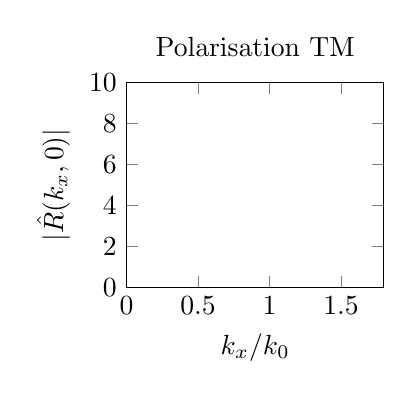
\begin{tikzpicture}[scale=1]
    \begin{axis}[
            title={Polarisation TM},
            ylabel={\(|\hat{R}(k_x,0)|\)},
            xlabel={\(k_x\slash k_0\)},
            width=0.4\textwidth,
            ymin=0,
            ymax=10,
            restrict y to domain=0:+4E+01,
            xmin=0,
            xmax=1.8,
            mark repeat=40,
            legend pos=outer north east
        ]
        % \addplot [color=black,mark=square*] table [col sep=comma, x={s1}, y={Abs(r_ex.tm)}] {csv/SOUDAIS/SOUDAIS.r_ex.MODE_2_TYPE_P.csv};
        % % \addlegendentry{Exact};

        % \addplot [color=blue,mark=x] table [col sep=comma, x={s1}, y={Abs(r_ibc0.tm)}] {csv/SOUDAIS/SOUDAIS.r_ibc.IBC_ibc0_SUC_F_MODE_2_TYPE_P.csv};
        % % \addlegendentry{CI0};

        % \addplot [color=red,mark=diamond*] table [col sep=comma, x={s1}, y={Abs(r_ibc3.tm)}] {csv/SOUDAIS/SOUDAIS.r_ibc.IBC_ibc3_SUC_F_MODE_2_TYPE_P.csv};
        % % \addlegendentry{CI3};
    \end{axis}
\end{tikzpicture}
\tikzsetnextfilename{R_SOUDAIS_plan_hoibc.TE}
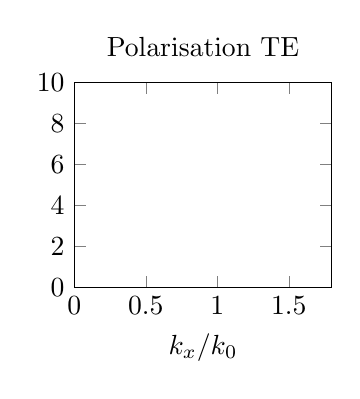
\begin{tikzpicture}[scale=1]
    \begin{axis}[
            title={Polarisation TE},
            ylabel={},
            xlabel={\(k_x\slash k_0\)},
            width=0.4\textwidth,
            xmin=0,
            xmax=1.8,
            ymin=0,
            ymax=10,
            mark repeat=40,
            legend pos=outer north east
        ]
        % \addplot [color=black,mark=square*] table [col sep=comma, x={s1}, y={Abs(r_ex.te)}] {csv/SOUDAIS/SOUDAIS.r_ex.MODE_2_TYPE_P.csv};
        % \addlegendentry{Exact};

        % \addplot [color=blue,mark=x] table [col sep=comma, x={s1}, y={Abs(r_ibc0.te)},color=] {csv/SOUDAIS/SOUDAIS.r_ibc.IBC_ibc0_SUC_F_MODE_2_TYPE_P.csv};
        % \addlegendentry{CI0};

        % \addplot [color=red,mark=diamond*] table [col sep=comma, x={s1}, y={Abs(r_ibc3.te)}] {csv/SOUDAIS/SOUDAIS.r_ibc.IBC_ibc3_SUC_F_MODE_2_TYPE_P.csv};
        % \addlegendentry{CI3};
    \end{axis}
\end{tikzpicture}
          \caption[CIOE sur empilement de P.~Soudais p.~11]{Module des coefficients diagonaux de \(\mR\) pour \(\eps = 4, \mu = 1, d=0.035\text{m}, f=12\text{GHz}\)}
          \label{fig:reflex_fourier:plan:soudais:hoibc}
      \end{figure}

      La figure \ref{fig:imp_fourier:plan:triple_asymptote:hoibc} montre la limite de la CI3 pour capturer 3 asymptotes. Pour cela, il faudrait utiliser une CI d'ordre au moins 6.

      L'expression de cette CIOE que l'on nomme \hyperlink{ci7}{CI7} est
      \begin{equation}
        \left(\oI + \sum_{i=1}^3 \left(d_{i} \left(\frac{\LD}{k_0^2}\right)^i + e_{i} \left(-\frac{\LR}{k_0^2}\right)^i \right)\right)\vE_t = \left(a_0 \oI + \sum_{i=1}^3 \left(b_{i} \left(\frac{\LD}{k_0^2}\right)^i + c_{i} \left(-\frac{\LR}{k_0^2}^i\right) \right)\right)\vJ
      \end{equation}

      \begin{figure}[!hbt]
          \centering
          \tikzsetnextfilename{Z_triple_asymptote_plan_hoibc_TM}
\begin{tikzpicture}[scale=1]
    \begin{axis}[
            title={Polarisation TM},
            ylabel={\(\Im(\hat{Z}(k_x,0)\)},
            xlabel={\(k_x\slash k_0\)},
            width=0.4\textwidth,
            xmin=0,
            xmax=1.999,
            ymin=-10,
            ymax=10,
            restrict y to domain=-300:300,
            mark repeat=200,
            legend pos=outer north east
        ]
        \addplot [color=black,mark=square*] table [col sep=comma, x={s1}, y={Im(z_ex.tm)}] {csv/triple_asymptote/triple_asymptote.z_ex.P.csv};
        % \addlegendentry{Exact};

        \addplot [color=blue,mark=x] table [col sep=comma, x={s1}, y={Im(z_ibc0.tm)}] {csv/triple_asymptote/triple_asymptote.z_ibc.IBC_ibc0_TYPE_P_SUC_F.csv};
        % \addlegendentry{CI0};

        \addplot [color=red,mark=diamond*] table [col sep=comma, x={s1}, y={Im(z_ibc3.tm)}] {csv/triple_asymptote/triple_asymptote.z_ibc.IBC_ibc3_TYPE_P_SUC_F.csv};
        % \addlegendentry{CI3};

        \addplot [color=cyan,mark=pentagon*] table [col sep=comma, x={s1}, y={Im(z_ibc7.tm)}] {csv/triple_asymptote/triple_asymptote.z_ibc.IBC_ibc7_TYPE_P_SUC_F.csv};
        % \addlegendentry{CI7};
    \end{axis}
\end{tikzpicture}
\tikzsetnextfilename{Z_triple_asymptote_plan_hoibc_TE}
\begin{tikzpicture}[scale=1]
    \begin{axis}[
            title={Polarisation TE},
            ylabel={},
            xlabel={\(k_x\slash k_0\)},
            width=0.4\textwidth,
            xmin=0,
            xmax=1.999,
            ymin=-10,
            ymax=10,
            restrict y to domain=-300:300,
            mark repeat=200,
            legend pos=outer north east
        ]
        \addplot [color=black,mark=square*] table [col sep=comma, x={s1}, y={Im(z_ex.te)}] {csv/triple_asymptote/triple_asymptote.z_ex.P.csv};
        \addlegendentry{Exact};

        \addplot [color=blue,mark=x] table [col sep=comma, x={s1}, y={Im(z_ibc0.te)}] {csv/triple_asymptote/triple_asymptote.z_ibc.IBC_ibc0_TYPE_P_SUC_F.csv};
        \addlegendentry{CI0};

        \addplot [color=red,mark=diamond*] table [col sep=comma, x={s1}, y={Im(z_ibc3.te)}] {csv/triple_asymptote/triple_asymptote.z_ibc.IBC_ibc3_TYPE_P_SUC_F.csv};
        \addlegendentry{CI3};

        \addplot [color=cyan,mark=pentagon*] table [col sep=comma, x={s1}, y={Im(z_ibc7.te)}] {csv/triple_asymptote/triple_asymptote.z_ibc.IBC_ibc7_TYPE_P_SUC_F.csv};
        \addlegendentry{CI7};                  
    \end{axis}
\end{tikzpicture}
          \caption[CIOE sur empilement avec triple asymptote]{Partie imaginaire des coefficients diagonaux de \(\mZ\) pour \(\eps = 4, \mu = 1, d=0.2\text{m}, f=1\text{GHz}\)}
          \label{fig:imp_fourier:plan:triple_asymptote:hoibc}
      \end{figure}
      \begin{table}[!hbt]
        \centering
        \begin{minipage}[t]{0.49\textwidth}
        \vspace{0pt}
        \centering
        \begin{coefftable}{\hyperlink{ci0}{CI0}}
          \input{csv/triple_asymptote/triple_asymptote.IBC_ibc0_SUC_F_MODE_2_TYPE_P.coeff.txt}
        \end{coefftable}

        \begin{coefftable}{\hyperlink{ci3}{CI3}}
          \input{csv/triple_asymptote/triple_asymptote.IBC_ibc3_SUC_F_MODE_2_TYPE_P.coeff.txt}
        \end{coefftable}
        \end{minipage}
        \tablecoeff[0.49]{\hyperlink{ci7}{CI7}}{csv/triple_asymptote/triple_asymptote.IBC_ibc7_SUC_F_MODE_2_TYPE_P.coeff.txt}
        \caption{Coefficients associés à la figure \ref{fig:imp_fourier:plan:triple_asymptote:hoibc}}
        \label{tab:imp_fourier:plan:triple_asymptote:hoibc}
      \end{table}
      Il faut donc une CIOE d'ordre 2 fois le nombre d'asymptote que l'on rencontre sur notre balayage.



\sectionstar{Conclusion}
Nous avons montré comment calculer les coefficients dans le cas d'un objet cylindre infini en minimisant au sens des moindres carrés la différence entre les coefficients de Fourier exact et approchés. 

Cette géométrie a pu montrer la limite de la CI3 pour approcher l'impédance exacte, mais qu'elle approchait bien les coefficients de la série de Fourier.
